\documentclass[format=sigconf, screen=true]{acmart}

%-------------- Customization of acmsmall package begins ----------------
\settopmatter{printacmref=false}%removes citation information below abstract
\renewcommand\footnotetextcopyrightpermission[1]{} 	% removes footnote with conference information in first column
\fancyfoot[LE,RO]{}									%removes footer with publication date
\fancypagestyle{firstpagestyle}{\fancyhf{}}			%removes footer with publication date on first page
\fancyhead[LE,RO]{\thepage}		%removes article number from header and leaves only page number
\makeatletter					%removes the black rectangle with article number
\renewcommand\@folioblob{}
\makeatother
%-------------- Customization of acmsmall package ends ----------------

\usepackage{thmtools}
\declaretheorem[style=acmdefinition,qed=$\vartriangleleft$,sibling=theorem,name=Example]{myexample}
\declaretheorem[style=acmplain,sibling=theorem]{remark}

%Import personal commands 
\usepackage{commandsrm}
%Load cleveref last
\usepackage[capitalize]{cleveref}

\usepackage{epigraph}
\setlength\epigraphwidth{8cm}
\setlength\epigraphrule{0pt}



% DOI
%\acmDOI{0000001.0000001}

\begin{document}
\title{Clever Title} 

\author{Alessandro Arlotto} 
\affiliation{Duke University}
\author{Siddhartha Banerjee}
\affiliation{Cornell University}
\author{Itai Gurvich}
\affiliation{Cornell University}
\author{Alberto Vera}
\affiliation{Cornell University}



\keywords{Online Stochastic Optimization, Prophet Inequalities, Approximate Dynamic Programming, Network Revenue Management, Online Packing.}
\begin{abstract}
\input{sec_abstract.tex}
\end{abstract}

\maketitle

\section{Introduction}

Overview:
\begin{enumerate}
\item Reason about a sequence of relaxations, as opposed to a single benchmark
\item Relaxations are random variables, not fixed values
\item They depend on revealing some information
\item Adversary is weakened in two ways: less information and has to process in the same order as online.
\item Study the sequence of relaxations with relaxed bellman equations
\item Predict the maximizers in the relaxed bellman eqs using an estimator of the relaxation
\end{enumerate}

\section{Relaxed Bellman Equations}
\section{Relaxed Bellman Equations}

Consider a DP with state space $\S$ and a sequence of inputs $\xit\in\Xi$ for $t\in[\T]$, where $t$ is the \emph{time to-go}.
We assume $\xit$ evolves as a Markov chain on state space $\Xi$, with known transition matrix and initial distribution.

For every state $s\in\S$, arrival $\xi$ and control $u\in\U$, we  collect a reward $\Re(s,\xi,u)$, which could be $-\infty$, and transition to the state $\Tr(s,\xi,u)$.
Observe that the reward function is deterministic, but the input $\xi$ is random, thus making the reward itself at each time a random variable.
We stress that, at each time $t$, the decision-maker first observes $\xit$ and based on that makes a decision.
\anote{
The only difference between this formulation and MCDP is that in MCDP the reward depends on a pair of states (current and transition), but I think that would be redundant.
}
Any time dependence will be embedded in the process $\xit$, e.g., if the randomness represents unknown demand, the state of the Markov chain could be of the form $\J=\crl{(t,x):t\in[\T],x\in\Rp}$, where the first component gives us the time and the second the demand for the period.
This formulation is known as a Markov Chance-Decision Process \cite[chap 13]{online_book}.

Given this formulation, if at time $t$ the current state is $s\in\S$, we obtain the Bellman \cref{eq:bellman_mcdp}
\begin{equation}\label{eq:bellman_mcdp}
v(t,s,\xit) = \max_{u\in\U}\crl{\Re(s,\xit,u) +\E_{\xi^{t-1}}[v(t-1,\Tr(s,\xit,u),\xi^{t-1})|\xit]},
\end{equation}
with boundary condition $v(0,\cdot,\cdot)=0$ and $\xi^0$ set to an arbitrary value.
This is a well-known fact; contingent on the actions being optimal, the total to-go value can be decomposed as instant reward plus future value.
We will now state a relaxed version of \cref{eq:bellman_mcdp}, where the main idea is to replace $v$, which is difficult to compute, for an efficiently computable upper bound $\tilde v$.
If $\tilde v$ satisfies a probabilistic version of a Bellman Equation, then the process of iteratively solving the relaxed problem can be justified.

\begin{definition}[Relaxed Bellman Equations]
The function $\varphi:[T]\times\S\times\Xi\to \R$ satisfies the relaxed Bellman equations w.r.t.\ $v$ if:
\begin{enumerate}
\item Initial condition: $\E[v(\T,S^\T,\xi^\T)] \leq \E[\varphi(\T,S^\T,\xi^\T)]$
\item Probabilistic inequality: $\forall s\in\S,t\in[T]$, there is a set $\calB(t,s)\subseteq\Omega$ such that
\begin{equation}\label{eq:relaxed_bellman}
\varphi(t,s,\xit) \leq \max_{u\in\U}\crl{R(s,\xit,u)+\E_{\xi^{t-1}}[\varphi(t-1,\Tr(s,\xit,u),\xi^{t-1})|\xit]} \quad \forall \omega\in\calB(t,s).
\end{equation}
\end{enumerate}
\end{definition} 
 
\begin{example}
Consider a knapsack problem with two types of stochastic arrivals.
Type $j$ has reward $r_j$, arrives at each period with probability $p_j$ and uses space $w_j$ in the knapsack.
Assume all the arrivals are revealed.
We will show that the following satisfies the relaxed Bellman equations:
\[
\varphi(t,b,\xit) = \max\crl*{\sum_{j}x_jr_j:\sum_{j}w_jx_j\leq b, \quad 0\leq x_j \leq Z_j(t) \quad \forall j\in[2]}.
\]
The initial condition is trivial, since we are relaxing the integrality constraints.
We are left to show the probabilistic inequality.
Let $X[\omega]$ be a solution to the LP and let $i=\xit$.
For the remainder of the example, we will assume $X_i\in(0,1)$.
If $Z_i(t)\geq 2$,  then an exchange argument shows
\[
\varphi(t,b,\xit) = \max_{u=\texttt{r,a}}\crl{r(b,\xit,u)+\varphi(t-1,b\ominus u,\xi^{t-1})}
= \varphi(t-1,b,\xi^{t-1}),
\]
where $b\ominus u$ denotes the natural reduction of budget of an action.
We conclude that, if $Z_i(t)\geq 2$ and $X_i<1$, the probabilistic inequality is satisfied a.s.
We are left with the case $Z_i(t)=1$ (the case $Z_i(t)=0$ is impossible when $X_i\in (0,1)$).
In this case, 
\[
\varphi(t,b,\xit) > \max_{u=\texttt{r,a}}\crl{r(b,\xit,u)+\varphi(t-1,b\ominus u,\xi^{t-1})}.
\]
We conclude that the probabilistic inequality is satisfied in $\calB(t,b)=\crl{\omega\in\Omega:Z_i(t)\geq 2}$.
Observe that the probability of this set is exponentially close to one.
Indeed, $\Pr[\calB(t,b)]=1-tp_i(1-p_i)^{t-1}$.
\end{example}

\begin{proposition}\label[proposition]{prop:relaxed_bellman}
Assume $\varphi$ satisfies the relaxed Bellman equations w.r.t.\ $v$.
Denote $\St$ the state of the policy that takes action $\Ut=\Ut(\xit,\St)$, where $\Ut$ is a maximizer in \cref{eq:relaxed_bellman}.
Then,
\[
\E[v(\T,S^\T,\xi^\T)] \leq \E\brk*{ \sum_{t=1}^\T (\Re(\St,\xit,\Ut)+\rmax\Ins{B(t,\St)})}. 
\]
\end{proposition}
\begin{proof}
By the initial condition property, $\E[v(\T,S^\T,\xi^\T)] \leq \E[\varphi(\T,S^\T,\xi^\T)]$.
It is now enough to argue the following equation and conclude by a simple induction step.
\[
\varphi(t,\St,\xit)\leq \E_{\xi^{t-1}}[\Re(\St,\xit,\Ut)+\varphi(t-1,S^{t-1},\xi^{t-1}) +  \rmax\Ins{B(t,\St)}|\xit].
\]
By definition of $\Ut$, $\varphi(t,\St,\xit)\leq \Re(\St,\xit,\Ut)+\E_{\xi^{t-1}}[\varphi(t-1,S^{t-1},\xi^{t-1})] +  \rmax\Ins{B(t,\St)}$.
Since $\Re(\St,\xit,\Ut)$ and $\Ins{B(t,\St)}$ are measurable with respect to $\xit$, they can be inside the expectation, showing that the desired equation holds.
\end{proof}

\anote{The $\rmax$ term here corresponds to the loss in $\varphi$.
All the relaxations we use have the same $\rmax$ as we would expect.}

\section{Probing}
High level description of the problem with no math. \todonote

\subsection{Formal Problem Statement}

At each time $t$, an arrival is drawn from a set of $n$ types with some known distribution.
Each type $j$ has a random reward drawn from the set $\crl{0,r_{j1},r_{j2}}$; we must make a decision after the type is revealed, but before observing the realized reward.
More precisely, type $j$ is associated with values $r_{j1},r_{j2}>0$ and probabilities $q_{j1},q_{j2}\in[0,1]$ such that $q_{j1}+q_{j2}\leq 1$.
The reward of a type $j$ is $r_{jk}$ with probability $q_{jk}$, $k\in\crl{0,1,2}$, where $r_{j0}\defeq 0$ and $q_{j0}\defeq 1-q_{j1}-q_{j2}$.

The decision-maker is given hiring and probing budgets $\Bh,\Bp\in\N$.
If he chooses to probe an arrival, then he can see the realization of the reward and then decide whether to accept or reject, thus probing protects against low realizations.
He can also choose to accept the arrival without probing, in such case the reward is random, but it does not consume probing budget.

Let us denote the average type $j$ reward by $\bar r_j\defeq r_{j1}q_{j1}+r_{j2}q_{j2}$.
It is instructive to consider extreme cases of $\Bp$.
If $\Bp=\T$, then \onl probes every single arrival, thus the problem corresponds to the multi-secretary with a different arrival distribution.
On the other hand, if $\Bp=0$, then the problem also corresponds to the multi-secretary with each type having reward $r_j$.
If $\Bp$ is any other value, then it is not clear what the interaction between the two budgets is in a good policy.

\subsection{Formulation as a MCDP}
We work in $2\T$ time steps.
At even times, the input reveals the type $j$ and at odd times it reveals the actual realization given probabilities $q_{jk}$
Let us define an \emph{input process} $(\xit)_{t\in[2\T]}$ as a Markov chain in the state space $[n]\cup\crl{(j,k):j\in[n],k=0,1,2}$.
The transition probabilities are given by $P_{j,(j,k)}=q_{jk}$, $P_{(j,k),j'}=p_{j'}$.
For $\xi^{2t-1}=(j,k)$ we define $r(\xi^{2t-1})=r_{jk}$.

The state space (see \cref{fig:probing_states}) can be described as  
\[
\S=\crl{(b_h,b_p),(b_h,b_p,\diamond):b_h,b_p\in\N,\diamond\in \crl{\texttt{a,p,r}}}.
\]
The component $\diamond$ indicates if we are in the accept, probe or reject stage.
There is never a $\diamond$ at times $2t$ and, at $2t-1$, feasible controls are different for distinct $\diamond$.

\begin{figure}
\centering
\scalebox{0.7}{%
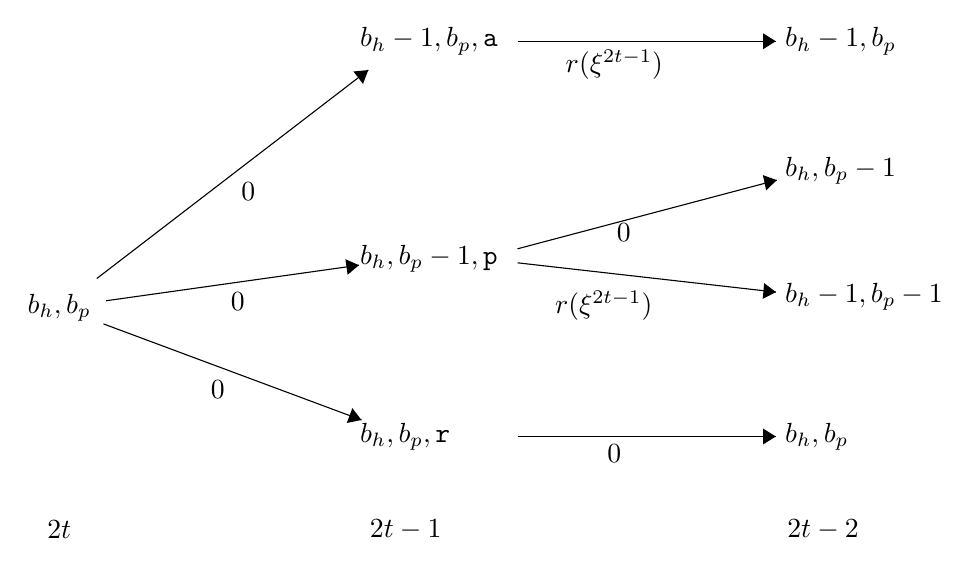
\begin{tikzpicture}[scale=0.2]
\tikzstyle{every node}+=[inner sep=0pt]

\draw (5.9,-25.9) node {$b_h,b_p$};

\draw (5.9,-40) node {$2t$};
\draw (27.9,-40) node {$2t-1$};
\draw (54.4,-40) node {$2t-2$};

\draw (30,-9) node[text width=2cm] {$b_h-1,b_p,\texttt{a}$};
\draw (30,-22.8) node[text width=2cm] {$b_h,b_p-1,\texttt{p}$};
\draw (30,-34.1) node[text width=2cm] {$b_h,b_p,\texttt{r}$};

\draw (57,-9) node[text width=2cm] {$b_h-1,b_p$};
\draw (57,-17.2) node[text width=2cm] {$b_h,b_p-1$};
\draw (57,-34.1) node[text width=2cm] {$b_h,b_p$};
\draw (57,-25.2) node[text width=2cm] {$b_h-1,b_p-1$};


\draw [black] (8.28,-24.07) -- (25.52,-10.83);
\fill [black] (25.52,-10.83) -- (24.58,-10.92) -- (25.19,-11.71);
\draw (17.91,-17.95) node [below] {$0$};
\draw [black] (8.87,-25.48) -- (24.93,-23.22);
\fill [black] (24.93,-23.22) -- (24.07,-22.84) -- (24.21,-23.83);
\draw (17.24,-24.94) node [below] {$0$};
\draw [black] (8.71,-26.95) -- (25.09,-33.05);
\fill [black] (25.09,-33.05) -- (24.51,-32.3) -- (24.16,-33.24);
\draw (15.97,-30.52) node [below] {$0$};

\draw [black] (35,-9) -- (51.4,-9);
\fill [black] (51.4,-9) -- (50.6,-8.5) -- (50.6,-9.5);
\draw (41.15,-9.5) node [below] {$r(\xi^{2t-1})$};
\draw [black] (35,-22.18) -- (51.46,-17.82);
\fill [black] (51.46,-17.82) -- (50.58,-17.5) -- (50.79,-18.47);
\draw (41.75,-20.58) node [below] {$0$};
\draw [black] (35,-23.07) -- (51.41,-24.93);
\fill [black] (51.41,-24.93) -- (50.66,-24.36) -- (50.57,-25.36);
\draw (40.47,-24.83) node [below] {$r(\xi^{2t-1})$};
\draw [black] (35,-34.1) -- (51.4,-34.1);
\fill [black] (51.4,-34.1) -- (50.6,-33.6) -- (50.6,-34.6);
\draw (41.15,-34.6) node [below] {$0$};
\end{tikzpicture}
}
\caption{Transitions for the online probing problem. 
Numbers below the arrows represent the reward of a transition.
At time $2t$ the possible actions are: accept, probe and reject.
At $2t-1$, depending on $\diamond$, we can either accept or reject and $b_h$ may be discounted.
}
\label{fig:probing_states}
\end{figure}


\subsection{Relaxation for Multiple Probing}

For every arrival we decide first whether to probe, reject or accept.
If we decide to probe, then there is a second decision, which uses the new information.
Say we observe type $j$ and $r_{j1}>r_{j2}>0$.
It is obvious that if the realization has zero reward we should reject.
An exchange argument shows that, if probing was optimal, then the value $r_{j1}$ must be accepted.
On the other hand, it is unclear if $r_{j2}$ should be accepted.
We must, therefore, reason about \off's actions at all times, instead of just at even times as before and concluding with structural properties.

Let $\calX\defeq\Rp^{7n}$ be the space for the decision variables.
In \cref{eq:probing_lp} we present a LP which will be the building block for our relaxation.
Note that, by definition, if $t$ is odd, $Z_j(t)=Z_j(t+1)-\In{\xi^{t+1}=j}$.

\begin{equation}\label{eq:probing_lp}
\begin{array}{rrll}
(P[t,b]) \; \max & \multicolumn{3}{l}{\sum_{j,k}r_{jk}x_{jka}+ \sum_j \bar r_jx_{ja}} \\
\text{s.t.}& \sum_{j,k}x_{jka}+\sum_jx_{ja} &\leq b_h  \\
&  \sum_j x_{jp} & \leq b_p   \\
&  x_{ja} +x_{jp} + x_{jr}&= Z_j(t)  & \forall j \\
& x_{jka} +x_{jkr} &= q_{jk}x_{jp} &  \forall j,k\\ 
& x&\in\calX.
\end{array}
\end{equation}

The LP in \cref{eq:probing_lp} can be interpreted as follows...\todonote

We are ready to parse the relaxation in \cref{eq:probing_relax}.
Recall that a state is of the form $s=(b_h,b_p,\diamond)$ with $\diamond\in \crl{\texttt{a},\texttt{p},\texttt{r},\varnothing}$, where $\diamond=\varnothing$ for even times.
The relaxation can be interpreted as giving \off the power to run a two-stage DP, where the value function is given by the corresponding LP.... \todonote
\begin{equation}\label{eq:probing_relax}
\varphi(t,s,\xit) = \left\{ 
\begin{array}{ll}
vP[t,b] & \diamond=\varnothing \\ 
vP[t-1,b] & \diamond = \texttt{r} \\ 
r_{\xit}+vP[t-1,b] & \diamond = \texttt{a} \\ 
\max\crl{r_{\xit}+vP[t-1,b-e_h],vP[t-1,Z,b]} & \diamond = \texttt{p}
\end{array} 
\right.
\end{equation}

We proceed to show that the relaxation satisfies the two conditions for the relaxed Bellman equations in \cref{def:relaxed_bellman}.
In \cref{lem:probing_initial} we show the initial condition and in \cref{lem:probing_ineq} the probabilistic inequality.


\anote{This is the proof for the active/inactive case. Need to update it}
\begin{lemma}\label[lemma]{lem:probing_initial}
For any $b_h,b_p\in\N$, $t\in[\T]$ and realization $Z$ of arrivals, $\voff(2T,b) \leq \varphi(2\T,(b,\varnothing),\xi^{2\T})$ 
\end{lemma}
\begin{proof}
Consider any policy for \off which determines when to probe, accept or reject.
The policy induces a random trajectory, which is determined by the realization of the Bernoulli variables, not the arrivals, since the later are given.
Define the following random variables, counting the number of times in which a type $j$: was probed, denoted $Y_j$; was accepted without probing, $X_{ja}$; and was accepted after probing, $X_{jp}$.
Finally, let $Y_{j}^+,X_{ja}^+$ be the number of active from among those probed or accepted, respectively.
We assume w.l.o.g.\ that, among the probed elements, \off takes only active ones.

Our aim is to argue that, replacing the aforementioned r.v.\ with their expectations, yields a feasible solution to $(P^\star)$.
It holds $\voff(t,b_h,b_p) = \E[\sum_j r_j(X_{jp}+X_{ja}^+)]$ and $\E[X_{ja}^+|X_{ja}]=q_jX_{ja}$, thus
\[
\voff(t,b_h,b_p) = \sum_jr_j(\E[X_{jp}]+q_j\E[X_{ja}]).
\] 

With the exception of the constraint $x_{jp}\leq q_jy_j$, $X_{ja},Y_j,X_{jp}$ satisfy a.s.\ all the constraints of $(P^\star)$, hence their expectations do too.
Observe that $X_{jp}\leq Y_{j}^+$ and $\E[Y_j^+]=q_j\E[Y_j]$, thus $\E[X_{jp}]\leq q_j\E[Y_j]$.
To summarize, $\voff(t,b_h,b_p)$ equals the value of the feasible solution given by the expectations, so $v(P^\star)$ can be only larger.
\end{proof}

\begin{lemma}\label[lemma]{lem:probing_ineq}
Let $\bar X\in\calX$ be a maximizer of $(P[t,b])$ for $t$ even.
Say $\xit=i$, then, at time $t$, \off is satisfied with the following actions:
\begin{enumerate}
\item Accept if $\bar X_{ia}\geq 1$
\item Reject $\bar X_{ir} \geq 1$
\item Probe if $\bar X_{ip}\geq 1$ and then accept $(i,k)$ if $\bar X_{(i,k)a}\geq 1$ or reject if $\bar X_{(i,k)r}\geq 1$
\end{enumerate}
\end{lemma}
\begin{proof}
We need to show the probabilistic inequality
\[
\varphi(t,s,\xit) \leq \max_{u\in\U}\crl{R(s,\xit,u)+\E_{\xi^{t-1}}[\varphi(t-1,\Tr(s,\xit,u),\xi^{t-1})|\xit]} \quad \forall \omega\in\calB(t,s).
\]
The set $\calB(t,s)$ is defined as the $\omega\in\Omega$ such that at least one of the conditions (1),(2) or (3) are satisfied.
Observe that, since $t$ is even, the instant reward $R(s,\xit,u)$ is zero.
In cases (1) and (2) is easy to verify the probabilistic inequality.
For case (3) we need to introduce some notation.
Let $\vec q_{j}\in\R^{2n}$ be a vector with value $q_{jk}$ in components $(j,k)$, $k=1,2$, and zero otherwise.
Similarly, let $\vec 1_{(j,k)}\in\R^{2n}$ have value $1$ in the single component $(j,k)$ and zero otherwise.
The following LP is the same as in \cref{eq:probing_lp}, but has an extra parameter to facilitate the analysis.
In particular, $vP[t,b]=v\bar P[t,b,0]$.

\begin{equation}
\begin{array}{rrll}
(\bar P[t,b,y]) \; \max & \multicolumn{3}{l}{\sum_{j,k}r_{jk}x_{jka}+ \sum_j \bar r_jx_{ja}} \\
\text{s.t.}& \sum_{j,k}x_{jka}+\sum_jx_{ja} &\leq b_h  \\
&  \sum_j x_{jp} & \leq b_p   \\
&  x_{ja} +x_{jp} +x_{jr} & \leq Z_j(t)  & \forall j \\
& x_{jka} +x_{jkr} &= q_{jk}x_{jp}+y &  \forall j,k.
\end{array}
\end{equation}

In case (3) we assume that the following holds: for every $k$, either $\bar X_{ika}\geq 1$ or $\bar X_{ikr}\geq 1$.
In other words, the LP wants to either fully reject one item or fully accept it.
With this assumption, denoting $I\defeq \In{\bar X(\xi^{t-1},a)\geq 1} $, we can write the following  a.s.\ equality (recall that $\xi^{t-1}$ is unknown at $t$)
\[
vP[t,b] = r_{\xi^{t-1}}I + v\bar P[t-1,b-e_p-e_hI,\vec q_{\xit}-\vec 1_{\xi^{t-1}}].
\]

In words, since $\bar X_{ip}\geq 1$, we can discount one in this variable when solving the LP, which reduces $b_p$ by $1$, $Z_j(t)$ by one and increases $y$ from $0$ to $\vec q_{i}$.
On the other hand, since either $\bar X_{ika}\geq 1$ or $\bar X_{ikr}\geq 1$, we can always discount $1$ from a single component $(i,k)$, which decreases $y$ by one in the corresponding component.
Finally, the indicators enforce that discounting from accept variables $\bar X_{ika}$ is preferable.

Now we can take expectations $\E[\cdot |\xit]$ and use Jensen's Inequality in only the variable $y$ of $\bar P$ as follows.
\begin{align*}
vP[t,b] &= \E[r_{\xi^{t-1}}I + v\bar P[t-1,b-e_p-e_hI,\vec q_{\xit}-\vec 1_{\xi^{t-1}}] |\xit] \\
&\leq \E[r_{\xi^{t-1}}I+ v\bar P[t-1,b-e_p-e_hI, 0] |\xit].
\end{align*}
Finally, since one of the options upper bounds $vP[t,b]$, surely the maximum does too, which is $\varphi(t-1,(b-e_p,\texttt{p}),\xi^{t-1})$.

\anote{What's going on is just a technical challenge. When we decide to probe at $t$, the right hand side does not go down by the same amount as the fluid does.
We need to justify that, in expectation you get a problem with a right hand side working in your favour.}
\end{proof}

Now we can invoke \cref{prop:relaxed_bellman} to conclude that \off is satisfied following the maximizers of our relaxation as long as fractional variables $(0,1)$ can be avoided.
Finally, we show how our policy approximates the solutions... \todonote

Consider the policy that, at even times solves $(P[t,\Bt])$, but with $Z(t)$ replaced by $\mu(t)\defeq \E[Z(t)]$ to get a solution $\Xt$.
Say $\xit=i$ is the current arrival.
If $\Xt_{ia}\geq \mu_{i}(t)/3$, the arrival is accepted.
Else if $\Xt_{ip} \geq \mu_i(t)/3$, the arrival is probed and then accepted contingent on $\Xt_{\xi^{t-1},a}\geq q_{\xi^{t-1}}\bar X_{ip}/2$.
Else, the arrival is rejected.

\begin{theorem}
The policy has regret bounded by a constant that depends on $n,q$ and the distribution of $Z(t)$ only.
\end{theorem}
\begin{proof}
Let $\Xts$ be a solution to $P[t,b]$.
In virtue of \cref{lem:probing_ineq}, if the policy accepts or rejects, the error is bounded by
\[
\Pr[\Xts_{i\diamond}<1|\Xt_{i\diamond}\geq \mu_i(t)/3], \quad \diamond=\texttt{a},\texttt{r}.
\]

If the policy probes, the error is bounded by the following, where $\diamond$ is the action with largest value between the variables $\Xt{\xi^{t-1},a},\Xt{\xi^{t-1},r}$.
\[
\Pr[\Xts_{ip}<1 \text{ or } \Xts_{\xi^{t-1},\diamond}<1|\Xt_{ip}\geq \mu_i(t)/3, \Xt_{\xi^{t-1},\diamond}\geq q_{\xi^{t-1}}\mu_i(t)/6 ]
\]

\anote{Now we can finish with the Lipschitz argument.
I'm not a big fan of it, because I'm still not sure if that's the best way to go about it, but it does abstract away all the technicalities in the deviations.

The exact regret bound would depend on the Lipschitz constant. I'm not sure how valuable it is to bound it more precisely.
}
\end{proof}

\section{Stochastic Knapsack With Frequentist Learning}
\paragraph{Problem Statement}
Items with known reward $r$ and random weight $W$ can be placed in a knapsack of capacity $B$.
At every time $t$, an arrival $j\in[n]$ is drawn with some known distribution, which generates a known reward of $r_j$.
The weight $W_j$ is a random variable, which is revealed only after the decision of accept/reject has been made.
The support of $W_j$ is known, but not the distribution.
An arrival can be accepted only if the weight is a.s.\ smaller than the remaining capacity.
At the end of each period, we observe the realization of both accepted and rejected items.

\off has access to the distribution of weights, \emph{but not to the realizations}.
Let $w_j\defeq \E[W_j]$ and $\Wt_j$ be the empirical average of the weights observed.
We assume that, before the process starts, we are given one sample of each weight type to initialize $\hat W_{jt}$.

Let $N_j(t)$ be the number of samples type $j$ observed at the beginning of $t$.
By definition we have $N_j(t)=Z_j(\T)-Z_j(t)+1$.
Following the same arguments, we can show that the relaxation in \cref{eq:knapsack_lp2} satisfies the initial condition.
\begin{equation}\label{eq:knapsack_lp2}
\begin{array}{rrll}
\varphi(t,b,\xit) \; = \; \max & \multicolumn{3}{l}{\sum_{j}r_{j}x_j} \\
\text{s.t.}& \sum_{j} w_jx_j  &\leq b  \\
&  x_j & \leq Z_j(t)  & j\in [n] \\
& x&\geq 0.
\end{array}
\end{equation}

Define as $\hat \varphi(t,b)$ the LP obtained from \cref{eq:knapsack_lp2} by replacing $Z_j(t)$ and $w_j$ by $\mu_j(t)\defeq\E[Z_j(t)]$ and $\Wt_j$, respectively.
Let $\sigma_j\in[n]$ be the rank of $j$ w.r.t.\ the ratio $r_j/w_j$, breaking ties lexicographically. 
For example, if $\sigma_j=1$, it means that $j$ is the most desirable item.
Similarly, $\sigmat_j$ denotes the rank of $j$ w.r.t.\ the ratio $r_j/\Wt_j$.

\begin{lemma}
Assume there are two items ($n=2$)  and $\abs{w_1-w_2}=\Delta>0$.
Let $\Xts,\Xt$ be the solutions to $\varphi,\hat\varphi$ respectively, then
\[
\Pr[\Xt_j\geq \mu_j(t)/2, \Xts<1] \leq STUFF, \quad 
\Pr[\Xt_j< \mu_j(t)/2, \Xts>Z_j(t)-1]\leq STUFF
\]
\end{lemma}
\begin{proof}
Let us bound the first probability by partitioning the space as
\[
\Pr[\Xt_j\geq \mu_j(t)/2, \Xts<1] \leq \Pr[\Xt_j\geq \mu_j(t)/2, \Xts<1, \sigma_j=\sigmat_j] + \Pr[\sigma_j\neq\sigmat_j].
\]
The term $\Pr[\sigma_j\neq\sigmat_j]$ decays with the number of samples $N_1(t),N_2(t)$.
We now bound the other term.

Say $j=1$ and let us study the case $\sigma_1=1$ first.
We can write $\Xts_1 = Z_1(t)\land \frac{b}{w_1}$ and $\Xt_1 = \mu_1(t)\land \frac{b}{\Wt_1}$.
Since we are assuming $\Xt_1\geq \mu_1(t)/2$, it follows that $\frac{b}{\Wt_1}\geq \mu_1(t)/2$.
On the other hand, $\Xts_1<1$ necessitates $\frac{b}{w_1}<1$ or $Z_1(t)=0$.
We can use these two inequalities to conclude
\[
\Pr[\Xt_j\geq \mu_j(t)/2, \Xts<1, \sigma_j=\sigmat_j=1] \leq \Pr[ w_1> \Wt_1 \mu_1(t)/2 \text{ or }  Z_1(t)=0].
\]
The probability of both events decay with $\mu_1(t)$.

Finally, let us study the case $\sigma_1=2$.
We can write $\Xts_2 = Z_2(t)\land \frac{b}{w_2}$, $\Xt_2 = \mu_2(t)\land \frac{b}{\Wt_2}$, $\Xts_1 = Z_1(t)\land \frac{b-\Xts_2w_2}{w_1}$ and $\Xt_1 = \mu_1(t)\land \frac{b-\Xt_2\Wt_2}{\Wt_1}$.
The conditions $\Xt_1\geq \mu_1(t)/2$ and $\Xts_1<1$ imply
\begin{align*}
& \Wt_1\frac{\mu_1(t)}{2}+\Xt_2\Wt_2\leq b < w_1+\Xts_2w_2 \quad \text{ or } \quad Z_1(t)=0\\
&\Longrightarrow \Wt_1\frac{\mu_1(t)}{2}< w_1+ (Z_2(t)w_2)\land b - (\mu_2(t)\Wt_2)\land b \quad \text{ or } \quad Z_1(t)=0 \\
&\Longrightarrow \Wt_1\frac{\mu_1(t)}{2}< w_1+ \abs{Z_2(t)w_2 -\mu_2(t)\Wt_2} \quad \text{ or } \quad Z_1(t)=0.
\end{align*}
For the last implication we used the fact that $x\land b - y\land b \leq \abs{x-y}$ holds for any reals $x,y,b$.
We conclude by observing that both events have probability decaying with $\mu_1(t),N_1(t),N_2(t)$.
\end{proof}

\section{Conclusions}
\input{sec_conclu.tex}


%% Bibliography
\bibliographystyle{plain}
\bibliography{biblio}

\end{document}
